% !TEX encoding = UTF-8 Unicode
%!TEX root = thesis.tex
% !TEX spellcheck = en-US
%%=========================================
\chapter{Introduction}
The first chapter of a well-structured thesis is always an introduction, setting the scene with background, problem description, objectives, limitations, and then looking ahead to summarize what is in the rest of the report. This is the part that readers look at first---\emph{so make sure it hooks them!}

%%=========================================
\section{Background}
In this section, you should present the problem that you are going to investigate or analyze; why this problem is of interest; what has, so far, been done to solve the problem, and which parts of the problem that remain.

{\color{red}Below, I have set up some headings (subsection titles) without a number. These are included to help you remember to cover the related issues. The headings should be removed in your final print.}
%%=========================================
\subsection*{Problem Formulation}
You should define your problem in a clear an unambiguous way and explain why this is a problem, why it is of interest---and to whom. It is also important to delimit the problem area.
%%=========================================
\subsection*{Related work}
You should here present the main books and articles that treat problems that are similar to what  you are studying, and give proper references to each of these as they are reported. If you,  later in your thesis, describe the ``state of the art'' -- with a detailed literature survey, you may just give a very brief survey here (approx. a quarter of a page). If this is the only literature survey, you need to go into more details. An objective of the literature survey is to show the reader that you are familiar with the main literature within your field of research -- so that you do not ``reinvent the wheel.''


References to literature can be given in two different ways:
\begin{itemize}
\item As an \emph{explicit} reference: It is shown by \citet{lundteigen08} and partly also by \citet{rausand14}  that \ldots.
\item As an \emph{implicit} reference: It is shown \citep[e.g., see][Chap. 4]{rausand04} that \ldots.
\end{itemize}
In the example above, we have used ``author-year'' references, which is the preferred format. 
\begin{remark}
Following agreement with your supervisor, you may also refer by numbers, for example,  [1]. To do this, open the file \texttt{ramsstyle.sty} and  comment out (by \%) the command \texttt{$\backslash$usepackage\{natbib\}} and un-comment the corresponding command \texttt{$\backslash$usepackage[numbers]\{natbib\}}.\footnote{Notice the strange way we have to write the ``backslash'' in the text. This is because the ``backslash'' is a command in \LaTeX.}
\end{remark}
 You may include a link to the Internet in the text or in a footnote by using a command like: \url{http://www.ntnu.edu/ross}. 

When you refer to the scientific literature, you should always write in \emph{present} tense. Example: \citet{rausand04} show that \ldots.

\begin{remark}
Hyperlinks are included by the command \texttt{$\backslash$usepackage\{hyperref}\} in \texttt{ramsstyle.sty}. If you feel that the hyperlinks are disturbing when you enter the text, or want to avoid the hyperlinks in printed text, you may either comment out or edit this command in \texttt{ramsstyle.sty}.
\end{remark}
%%=========================================
\subsection*{What Remains to be Done?}
After you have defined and delimited your problem -- and presented the relevant results found in the literature within this field, you should sum up which parts of the problem that remain to be solved.
%%=========================================
\section{Objectives / Research Questions}
The main objectives of this Master's project are
\begin{enumerate}
\item This is the first objective
\item This is the second objective
\item This is the third objective
\item More objectives
\end{enumerate}

The objectives shall be written as \emph{fundamental objectives} telling what to do and not \emph{means objectives} telling how to do it.

All objectives shall be stated such that we, after having read the thesis, can see whether or not you have met the objective. ``To become familiar with \ldots'' is therefore not a suitable objective.

%%=========================================
\section{Approach}
Here you should describe the (scientific) approach and experiments that you will use or have used to solve the problem and meet your objectives and tasks. Experiments may in this context relate analyses you need to carry out in order to investigate a specific hypothesis, task objective, or similar. You should specify the approach and experiments for each objective and/or task. It is preferred that you supplement your explanation of the approach with an illustration.

If there are any ethical problems related to your approach, these should be highlighted and discussed.

\subsection*{Research method}

\begin{wrapfigure}{r}{0.50\textwidth}
    \begin{center}
        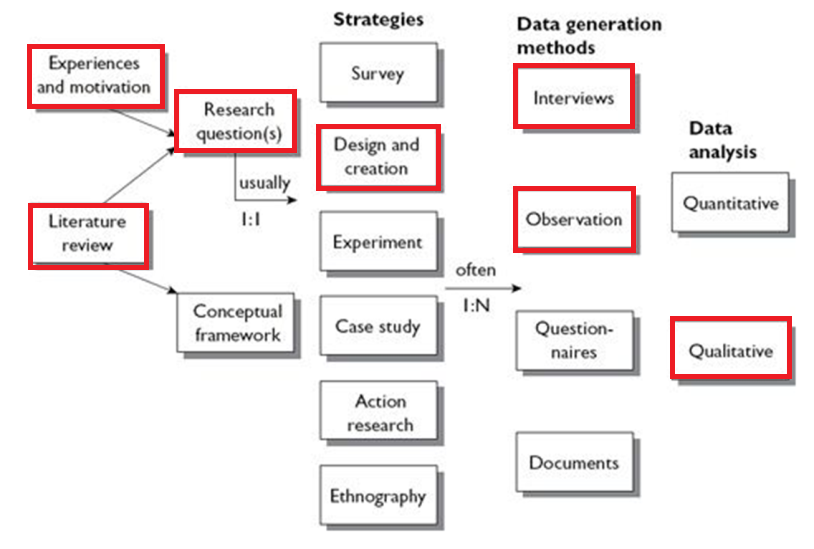
\includegraphics[width=0.48\textwidth]{fig/researchplan_image}
    \end{center}
    \caption{Model of the research process as illustrated in TODO: ref }
    \label{researchplan_img}
\end{wrapfigure}

The research questions were derived through discussing the needs of the intended users with neuroscientists at the Kavli Institute. It was then narrowed down by a literature review, finding a lack of satisfactory substitutions for real brain dissections and especially finding no attempt at a practical multiplatform application for a more scalable use for students. The projects research question falls under the strategy of Design and Creation as the main goal is to develop a useful application for medical education. The focus on a smartphone solution was further motivated by the COVID-pandemic making from-home learning quite essential and making the passing around of HMD devices an unwanted scenario. As part of an agile software development model the gathering of qualitative data from observations and interviews within the scope of user testing will be essential. 

\subsection*{Development method}

\section{Contributions}
%% write about macro vs micro stuff

The research product resulting from this project will be a new computer-based software application using augmented reality and running on multiple platforms like HoloLens 1 and 2, Android and more. The aim will be to develop an application that can bridge the gap between expensive head mounted displays and everyday smartphones which you will find in the pocket of any student, and to use this as a collaborative tool for learning neuroanatomy. Throughout the development period we will consult with medical professionals and gather feedback from students on the usability of the application.

%%=========================================
\section{Limitations}
In this section you describe the limitations of your study. These may be related to the study object (physical limitations, operational limitations), to the environmental and operational conditions, to the thoroughness of the analysis, and so on.

%%=========================================
\section{Outline}
Here, you give an overview of how the remaining part of the report is organized. A proposed structure of the main chapters in the report can be as follows (note that some chapters are not numbered):
\begin{itemize}
\item Preface: Contains practical information about what you have done, and where the work has been carried out. Any assumed background of the reader should be specified here.
\item Acknowledgments: Here, you show the gratitude to who have been supporting your work, professionally and family as relevant.
\item Summary: Contains the management summary, and should be a layman's explanation of what you have done and why it is important. This would be the talk you could give if you in an  interview is asked about what you did in your thesis, or if some of your relatives ask the same question. This chapter should therefore include as few domain specific words as possible, so that no detailed background in the topic is required. 
\item Chapter 1. Introduction: Structure already discussed in this chapter.
\item Chapter 2. Theoretical background: Here you identify and give the theoretical background needed in this report, with proper references to each literature reference used. The selection of what to include should be discussed and agreed with the supervisors. Theory may involve concepts, definitions, methods, regulations/key standards, theory to explain specific system behavior, and so on.
\item Chapter 3..N-2: The naming of the following chapters relies entirely on the specific topic in question. Proposed structure should be discussed with supervisor.
\item Chapter N-1 Results: This chapter should be the last chapter \textit{before} ``Conclusions, discussion, and ideas for further work''
\item Chapter N. Conclusions, discussion, and ideas for further work.
\item Bibliography
\item Appendix A etc (as needed): Appendix A may for example be acronyms as shown here.
\end{itemize}



\begin{remark}
Notice that chapter and section headings shall be written in lowercase, but that all main words should start with a capital letter.
\end{remark}



The report should be no longer than \underline{60 pages} in this format for the master as well as the specialization project, with the possible exception of appendixes (which may take up some space if including e.g. code from programming). This does not mean that the report must be at least 60 pages, and the effort should be directed to be as concise as possible throughout the report.